\chapter{Análise Bibliográfica sobre o uso da Inteligência Artificial em autonomia, por Conrado Nunes\label{chap:bibliometria:Conras21}}

\section{Planejamento do estudo}

Ultimamente a necessidade de soluções tecnológicas tem crescido bastante. A tecnologia da informação é uma área em constante crescimento, e dentre as diversas ramificações, a inteligência artificial vem tendo sua participação significativa nas soluções tecnológicas. A IA está presente no nosso dia a dia mesmo que não seja percebida, seja em algoritmos de sugestão, até em carros que dirigem de forma totalmente autônoma.

Algumas empresas como a tesla, uber, e etc vem investimento na autonomia dos carros, um carro que dirige de forma totalmente autônoma sem interferência humana. Em alguns estados dos EUA já está sendo testado o transporte de passageiros com esses carros.

\subsection{O que já existe de pesquisa bibliométrica sobre esse tema?}

A inteligência artificial pode ser usada em várias áreas diferentes, por esse motivo existem várias pesquisas para suas respectivas áreas.

\subsection{Uso do Bibliometrix e Biblioshiny}
Serão usadas a ferramenta e o \textit{workflow} proposto pelos autores do pacote Bibliometrix, conforme indica a figura ~\ref{fig:bibliometrix:workflow}.

\subsection{Limitações} O exercício relatado foi feito em apenas uma semana, envolvendo entre 5 a 10 horas de trabalho.


\begin{itemize}
\item O objetivo é exercitar inicialmente, e relatar, o uso da técnica de análise bibliométrica, para fins didáticos.
\end{itemize}


\section{Coleta de dados}

A coleta de dados feita usando o WoS no dia 02 de fevereiro de 2021, acessado por meio do Portal de Periódicos da CAPES.

Foram feitas buscas nas coleções Science  Citation  Index  Expanded (SCI -EXPANDED) e Social  Sciences  Citation  Index (SSCI), que contém registros relativos a vários campos do conhecimento, no qual o SCI-EXPANDED foca mais na área das ciências exatas e naturais, enquanto que o SSCI indexa artigos da área das ciências sociais. Observe que os artigos nessas duas coleções são indexados desde 1945. 

Essa busca consiste em dois termos, sendo que o primeiro é composto por Inteligência Artificial e o segundo pela palavra autonomia. Foram encontrados 1012 registros, para este trabalho utilizaremos os 1000 primeiros registros, disponíveis em \ref{}.

Foi usada a \textit{query} de busca ilustrada na listagem:

\lstinputlisting[numbers=left,basicstyle=\normalsize\ttfamily,caption={Query de busca sobre inteligencia artificial}]
{experiments/Conras21/queries/query.txt}


\section{Análise dos dados}

\subsection{Análise descritiva}


O bibliometrix, por meio da interface biblioshiny permite extrair uma tabela contendo as principais informações sobre os artigos contidos no IA@Conras21, abaixo estão listadas algumas dessas informações:
\begin{description}
    \item[Timespan] os artigos do \textit{dataset} IA@Conras21 abrangem os anos de 1991 a 2022, mostrando que o estudo da autonomia com inteligencia artificial e relativamente recente.
    \item[Sources (Journals, Books, etc)] há 322 fontes de informação no \textit{dataset} EDM@pedro-maschio.
    \item[Documents] há 4700 documentos no \textit{dataset} IA@Conras21, sendo todos artigos científicos.
    \item[Average years from publication] a média de anos de publicação do \textit{dataset} IA@Conras21 é de 6.1.
    \item[Average citations per documents] a média de citações por documento é de 16.12 no \textit{dataset} IA@Conras21.
    \item[Average citations per year per doc] a média de citações por ano por documento é de 2.266 no \textit{dataset} IA@Conras21.
    \item[References] há 29953 referências no \textit{dataset} IA@Conras21.
    \item[Authors] há 2609 nomes de autores distintos
    \item[Author Appearances] os 2609 autores distintos aparecem 2999 vezes
    \item[Authors of single-authored documents] 53 autoes publicaram artigos sem co-autores
    \item[Authors of multi-authored documents] 2556 autores foram autores de artigos em conjunto com outros autores.
    \item[Single-authored documents] 54 artigos foram escritos por um único autor
    \item[Documents per Author] a taxa de documentos por autor é de 0.287
    \item[Authors per Document] a taxa de autor por documento é de 3.48
    \item[Co-Authors per Documents] há em média 4 autores por artigos
    \item[Collaboration Index] o índice de colaboração é de 3,68
\end{description}

\section{Visualização dos dados}

\subsection{Evolução da produção Científica}

\begin{figure}[H]
    \centering
    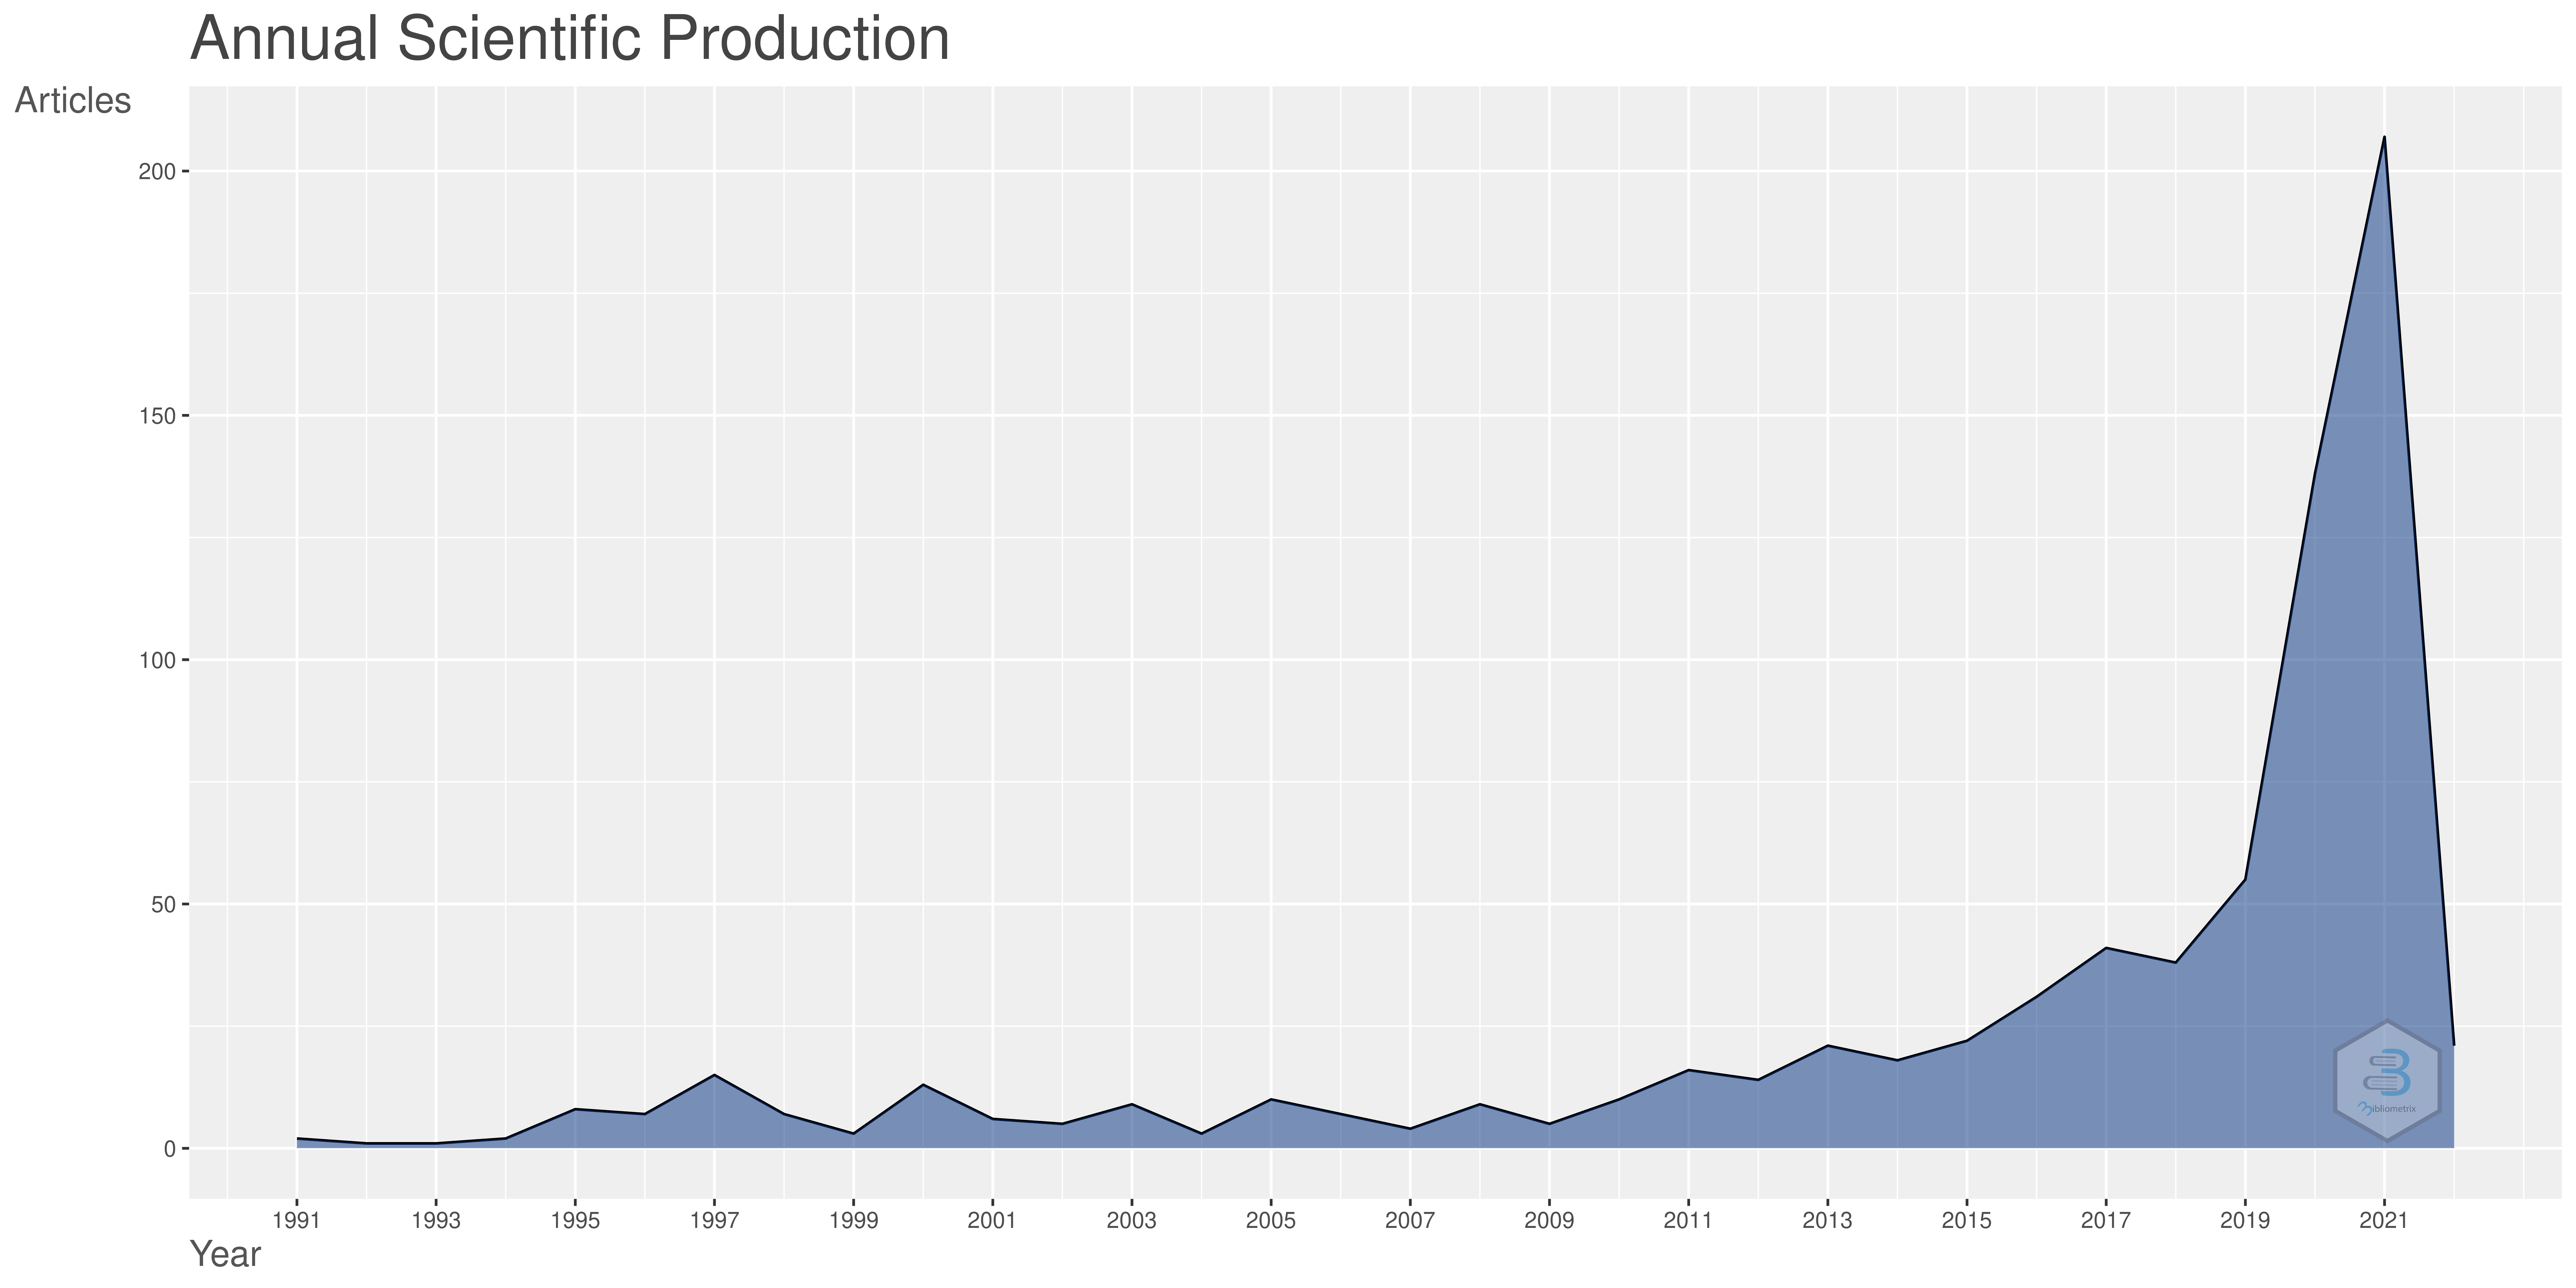
\includegraphics[width=1\textwidth]{experiments/Conras21/PesqBib/AnnualScientificProduction-2022-02-08.png}
    \caption{Evolução da produção científica no \textit{dataset} IA@Conras21.}
    \label{fig:evol:anual:IA@Conras21}
\end{figure}

Conforme apresenta-se na Figura \ref{fig:evol:anual:IA@Conras21}, a produção de artigos a respeito de inteligencia artificial cresceu bastante em 2021. O cresciemtno anual foi de 7.88\%. 

\subsection{Citações média por ano}

\begin{figure}[H]
    \centering
    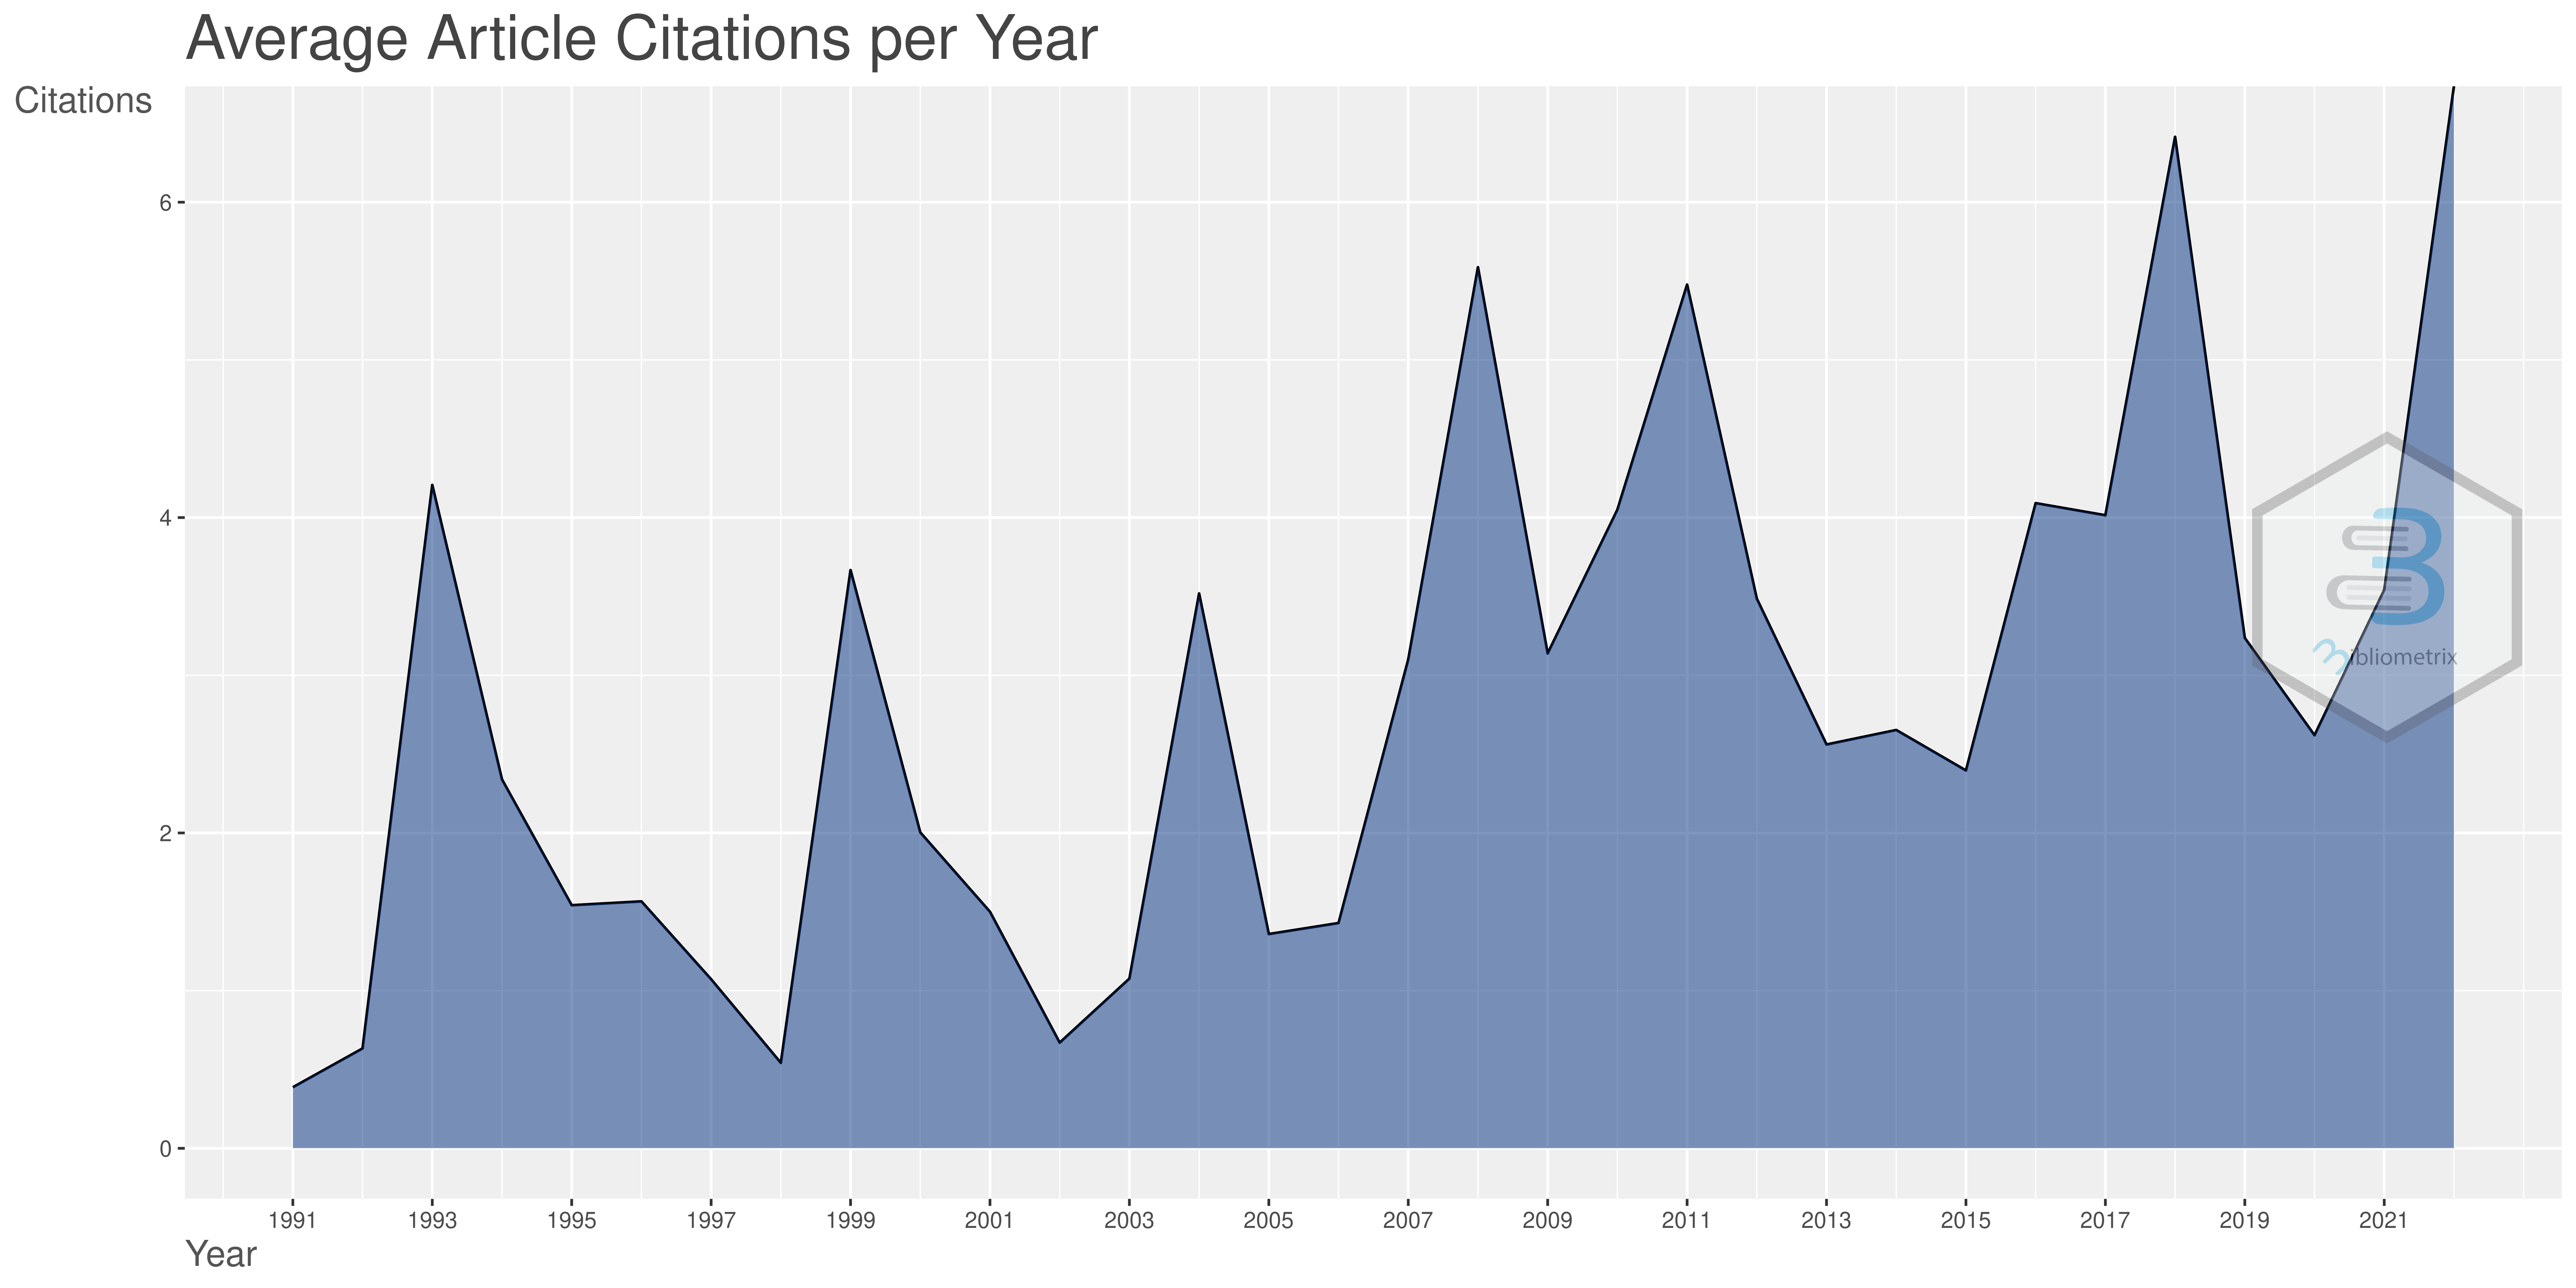
\includegraphics[width=1\textwidth]{experiments/Conras21/PesqBib/AverageArticleCitationPerYear-2022-02-08.png}
    \caption{Evolução da produção científica no \textit{dataset} IA@Conras21}
    \label{fig:citacoes:anual:IA@Conras21}
\end{figure}

Além da evolução no número de artigos publicados por ano, é possível extrair a evolução do número de citações média por ano, conforme apresenta-se na Figura \ref{fig:citacoes:anual:IA@Conras21}. 

\section{Resultados e interpretação}

Esta pesquisa bibliográfica indicou uma crescente busca de aprofundamento a respeito da inteligencia artificial, principalmente ligada a deep learning, principalmente no ano de 2020 em diante.